\section{Ergebnisse}
\label{sec:ergebnisse}

\subsection{Abdeckung und Overlap}
\label{subsec:ergebnisse_abdeckung}

Der Datensatz umfasst nach Bereinigung, Bot-Filterung und Beschränkung auf den Zeitraum ab dem 01.\,01.\,2026 insgesamt 2\,266 Tweets von 12 Fokus-Tickern. Nach Zusammenführung mit den historischen Tagespreisen ergaben sich 290 tatsächlich nutzbare, gepaarte Beobachtungen. Der überlappende Zeitraum erstreckte sich vom 02.\,01.\,2026 bis zum 23.\,04.\,2026.

Tabelle~\ref{tab:overlap} zeigt die Abdeckung je Ticker sowie die Eignung für die vier Analysemethoden. TSLA, VWAGY, XOM und BYDDY erfüllten alle Mindestanforderungen. BP und TTE hatten ausreichend Beobachtungen für Pearson/Spearman und die Event-Study, nicht aber für Rolling-Korrelation und Granger-Test. Für die übrigen Ticker konnten nur vereinzelte Korrelationskoeffizienten berechnet werden.

\begin{table}[H]
\centering
\caption{Overlap-Report: Abdeckung und Methoden-Eligibility je Fokus-Ticker}
\label{tab:overlap}
\begin{tabular}{lrcccc}
\toprule
\textbf{Ticker} & \textbf{Aligned Days} & \textbf{Corr} & \textbf{Rolling} & \textbf{Granger} & \textbf{Event} \\
\midrule
TSLA      & 68 & \checkmark & \checkmark & \checkmark & \checkmark \\
VWAGY     & 53 & \checkmark & \checkmark & \checkmark & \checkmark \\
XOM       & 41 & \checkmark & \checkmark & \checkmark & \checkmark \\
BYDDY     & 34 & \checkmark & \checkmark & \checkmark & \checkmark \\
BP        & 27 & \checkmark & --         & --         & \checkmark \\
TTE       & 23 & \checkmark & --         & --         & \checkmark \\
6503.T    & 17 & \checkmark & --         & --         & --         \\
6367.T    & 11 & \checkmark & --         & --         & --         \\
E         &  7 & \checkmark & --         & --         & --         \\
SHEL      &  5 & \checkmark & --         & --         & --         \\
CARR      &  3 & --         & --         & --         & --         \\
NIBE-B.ST &  1 & --         & --         & --         & --         \\
\bottomrule
\multicolumn{6}{l}{\footnotesize \checkmark = Methode anwendbar; -- = Mindestanforderung nicht erfüllt}
\end{tabular}
\end{table}

% ─────────────────────────────────────────────────────────────────────────────
\subsection{Sentiment-Verteilung}
\label{subsec:ergebnisse_sentiment}

\begin{figure}[H]
  \centering
  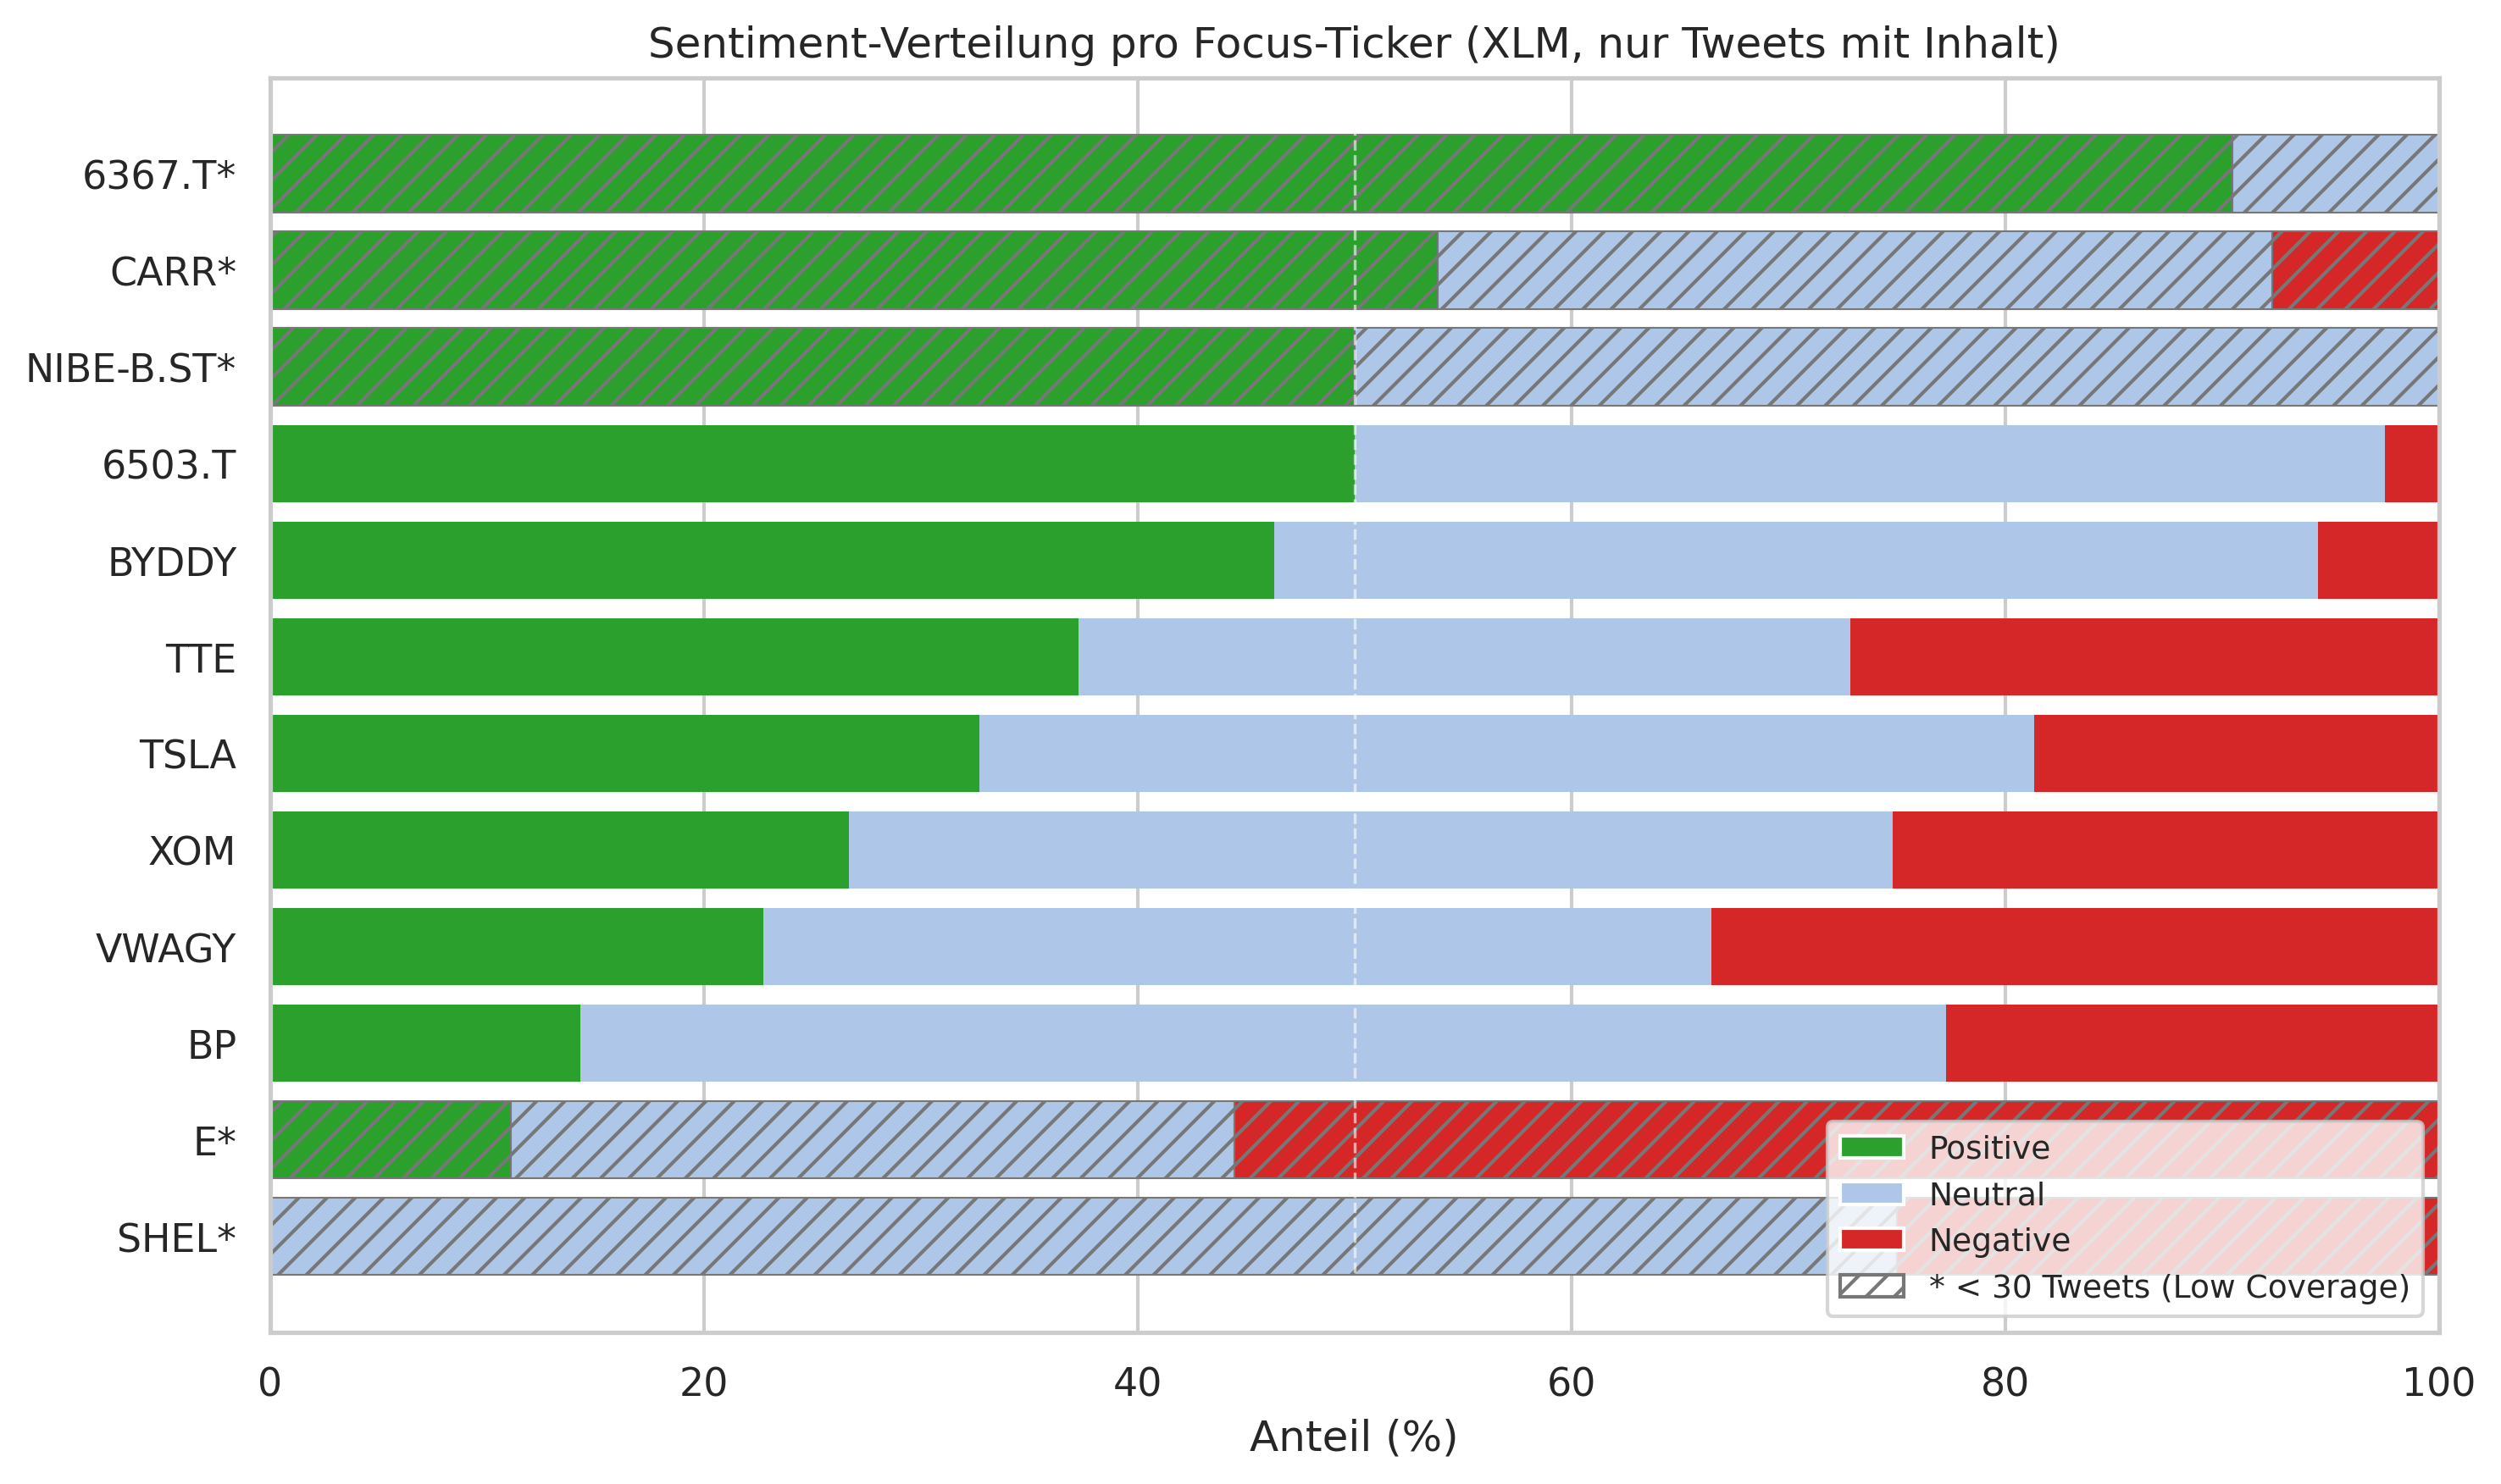
\includegraphics[width=0.85\textwidth]{figures/02_sentiment_analysis/02_sentiment_distribution_by_ticker.png}
  \caption{Sentiment-Verteilung pro Fokus-Ticker (XLM-RoBERTa, nur Tweets mit substantiellem Inhalt). Schraffierte Balken markieren Ticker mit weniger als 30 Tweets (niedrige Abdeckung).}
  \label{fig:label_distribution}
\end{figure}

Über alle Fokus-Ticker verteilt zeigte das XLM-RoBERTa-Modell folgende Labelverteilung: rund 31,9\,\% der verwertbaren Tweets wurden als positiv, 48,5\,\% als neutral und 19,6\,\% als negativ klassifiziert. Der mittlere XLM-Compound-Score auf Tagesaggregat-Ebene betrug $\bar{s} = 0.13$ mit einer Standardabweichung von $\sigma = 0.41$, was auf ein insgesamt leicht positives, aber stark streuendes Signal hindeutet.

Die Übereinstimmung zwischen XLM-RoBERTa und VADER über alle Sprachen betrug 56{,}9\,\% und stieg für den englischsprachigen Teilkorpus auf 57{,}0\,\% an (vgl.\ Abb.~\ref{fig:xlm_vader_scatter}). Der geringe Anstieg beim englischen Teilkorpus deutet darauf hin, dass die sprachliche Homogenisierung allein keinen wesentlichen Unterschied macht; grundlegend unterschiedliche Modellarchitekturen und Trainingskorpora bleiben die Hauptursache für Abweichungen.

\begin{figure}[H]
  \centering
  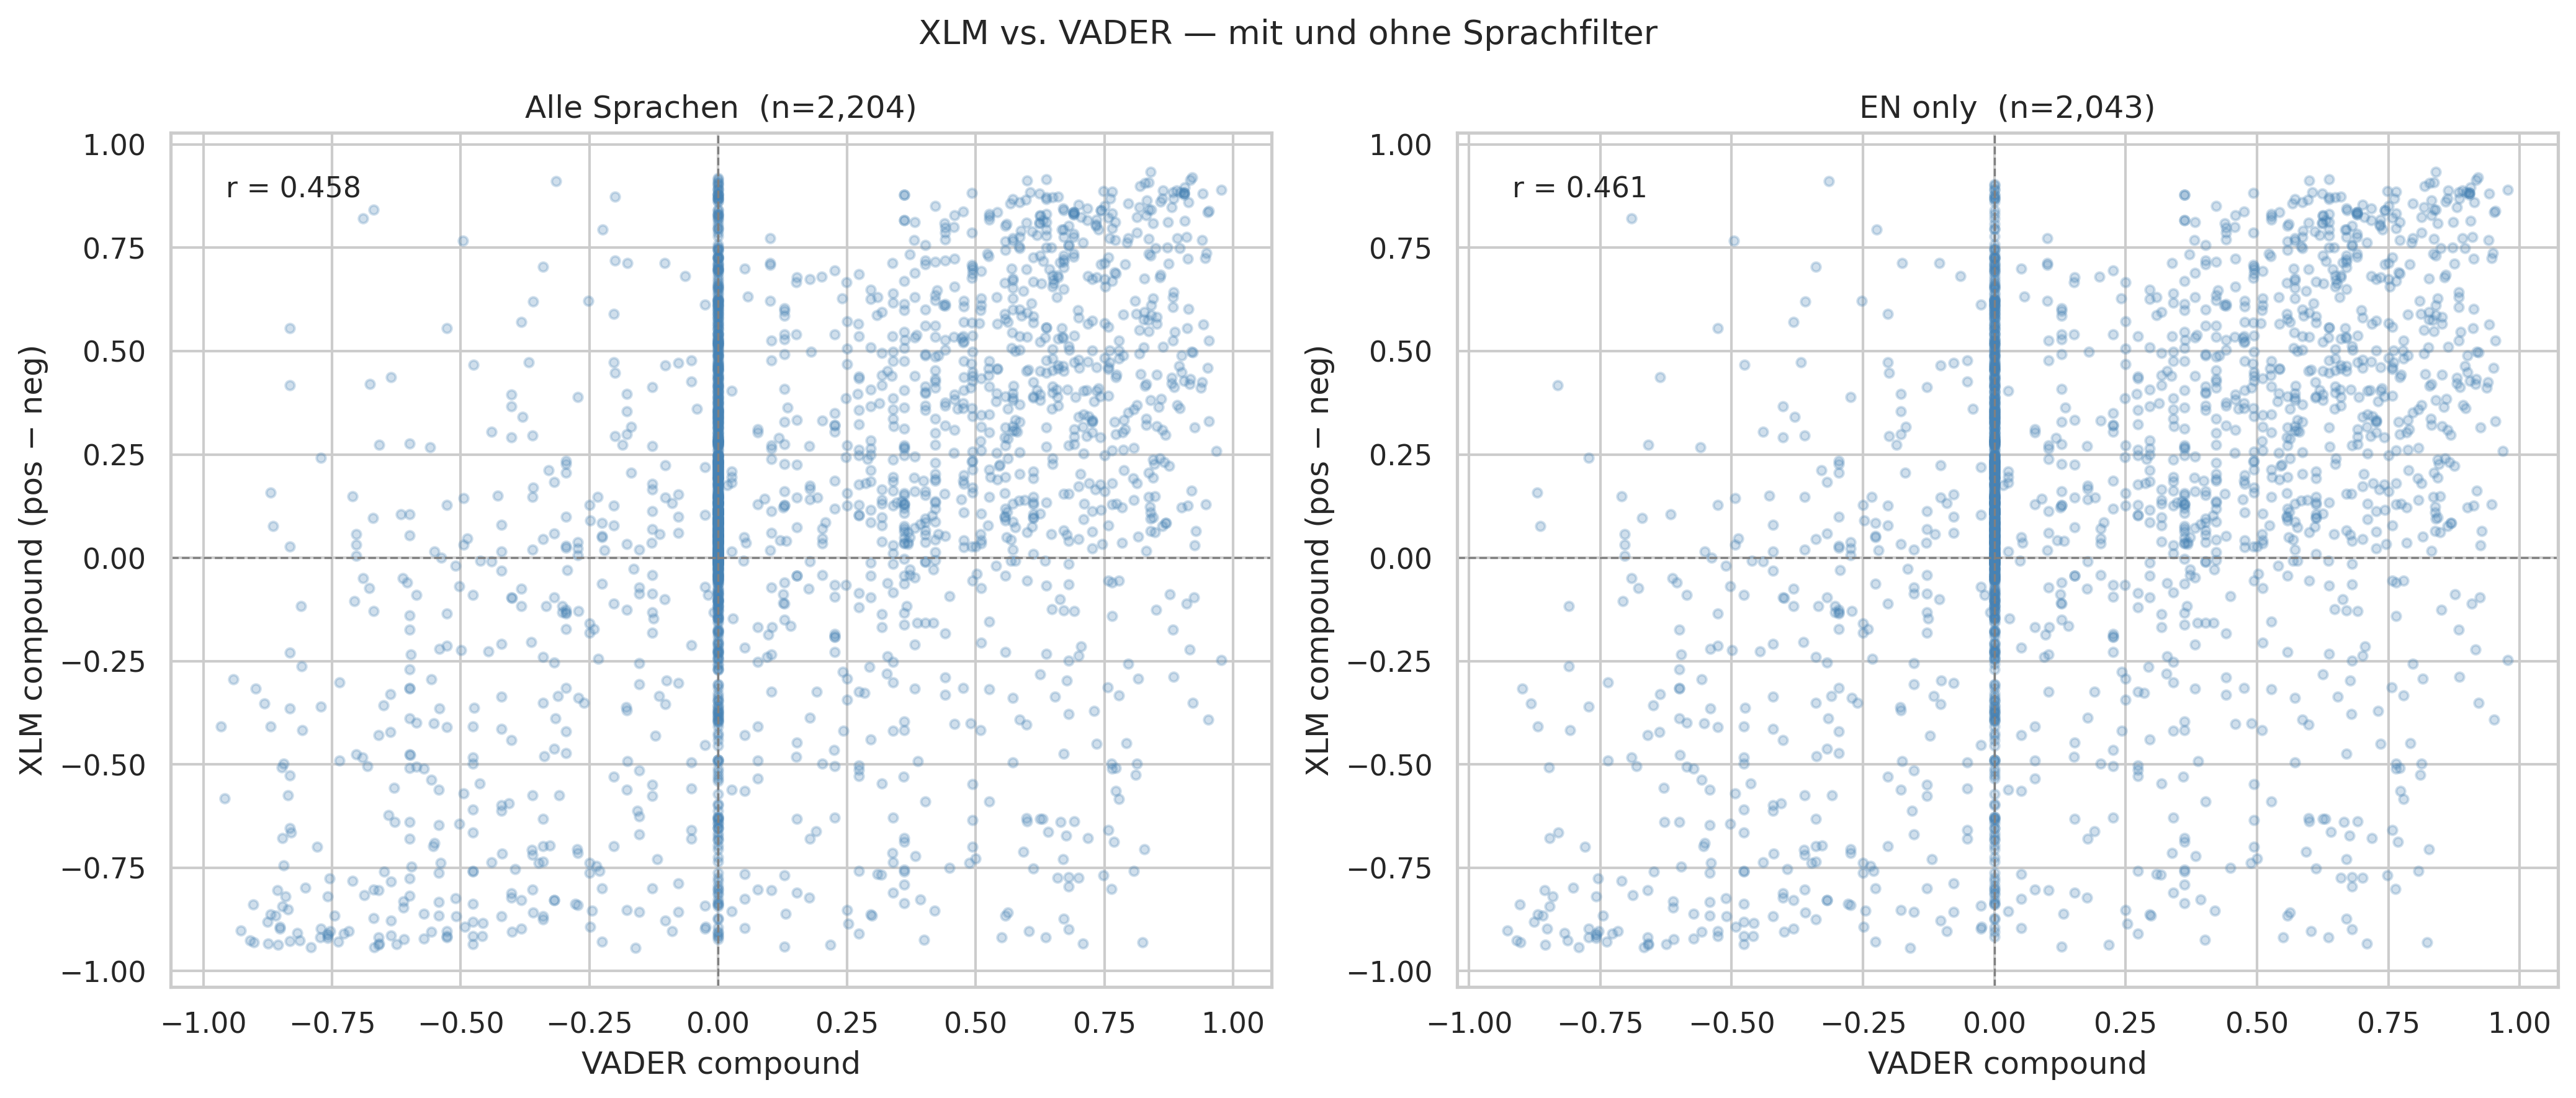
\includegraphics[width=\textwidth]{figures/02_sentiment_analysis/01_xlm_vs_vader_scatter.png}
  \caption{Streudiagramm XLM-RoBERTa- vs.\ VADER-Compound-Score: links alle Sprachen ($n=2\,204$), rechts nur englischsprachige Tweets ($n=2\,043$). Der Pearson-Korrelationskoeffizient $r$ ist jeweils angegeben.}
  \label{fig:xlm_vader_scatter}
\end{figure}

% ─────────────────────────────────────────────────────────────────────────────
\subsection{Lag-Korrelation}
\label{subsec:ergebnisse_lagkorr}

Tabelle~\ref{tab:lag_corr} fasst die stärksten Pearson-Korrelationen je Ticker über alle Lags zusammen.

\begin{table}[H]
\centering
\caption{Stärkste Lag-Korrelationen (Pearson $r$) je Fokus-Ticker mit dem follower-gewichteten Sentiment-Signal. 95\,\%-KI via Fisher-$z$-Transformation. $p_{\mathrm{adj}}$ nach Benjamini-Hochberg-Korrektur.}
\label{tab:lag_corr}
\begin{tabular}{lrrrrrr}
\toprule
\textbf{Ticker} & \textbf{Bester Lag} & \textbf{Pearson $r$} & \textbf{95\,\%-KI} & \textbf{$p_{\mathrm{roh}}$} & \textbf{$p_{\mathrm{adj}}$} & \textbf{$n$} \\
\midrule
E        & Lag 2 & $-0.762$ & $[-0.983,\;+0.367]$ & 0.134 & 0.830 & 5  \\
6367.T   & Lag 1 & $-0.636$ & $[-0.904,\;-0.011]$ & 0.048 & 0.830 & 10 \\
TTE      & Lag 0 & $+0.294$ & $[-0.135,\;+0.630]$ & 0.174 & 0.830 & 23 \\
6503.T   & Lag 0 & $-0.283$ & $[-0.672,\;+0.229]$ & 0.272 & 0.830 & 17 \\
BYDDY    & Lag 3 & $-0.237$ & $[-0.546,\;+0.128]$ & 0.198 & 0.830 & 31 \\
TSLA     & Lag 0 & $-0.234$ & $[-0.447,\;+0.005]$ & 0.055 & 0.830 & 68 \\
XOM      & Lag 3 & $-0.232$ & $[-0.513,\;+0.095]$ & 0.162 & 0.830 & 38 \\
VWAGY    & Lag 3 & $+0.220$ & $[-0.062,\;+0.469]$ & 0.125 & 0.830 & 50 \\
BP       & Lag 0 & $-0.212$ & $[-0.548,\;+0.183]$ & 0.289 & 0.830 & 27 \\
SHEL     & Lag 0 & $+0.196$ & $[-0.830,\;+0.919]$ & 0.752 & 0.952 &  5 \\
\bottomrule
\multicolumn{7}{l}{\footnotesize Kein $p_{\mathrm{adj}} < 0{,}05$ nach BH-FDR-Korrektur (40 Tests gesamt)}
\end{tabular}
\end{table}

Kein Koeffizient blieb nach Anwendung der Benjamini-Hochberg-Korrektur für multiples Testen signifikant ($p_{\mathrm{adj}} < 0{,}05$). Ohne Korrektur wies lediglich 6367.T\,(Daikin) auf Lag~1 einen rohen $p$-Wert unter 0,05 auf ($r = -0.636$, $p_{\mathrm{roh}} = 0.048$, $p_{\mathrm{adj}} = 0.830$). Das breite 95\,\%-Konfidenzintervall dieses Koeffizienten von $[-0.904, -0.011]$ bei $n = 10$ Beobachtungen verdeutlicht die erhebliche Schätzunsicherheit. Dieser Befund ist als zufälliger Treffer bei 40 simultanen Tests zu bewerten und daher nicht inhaltlich interpretierbar.

\begin{figure}[H]
  \centering
  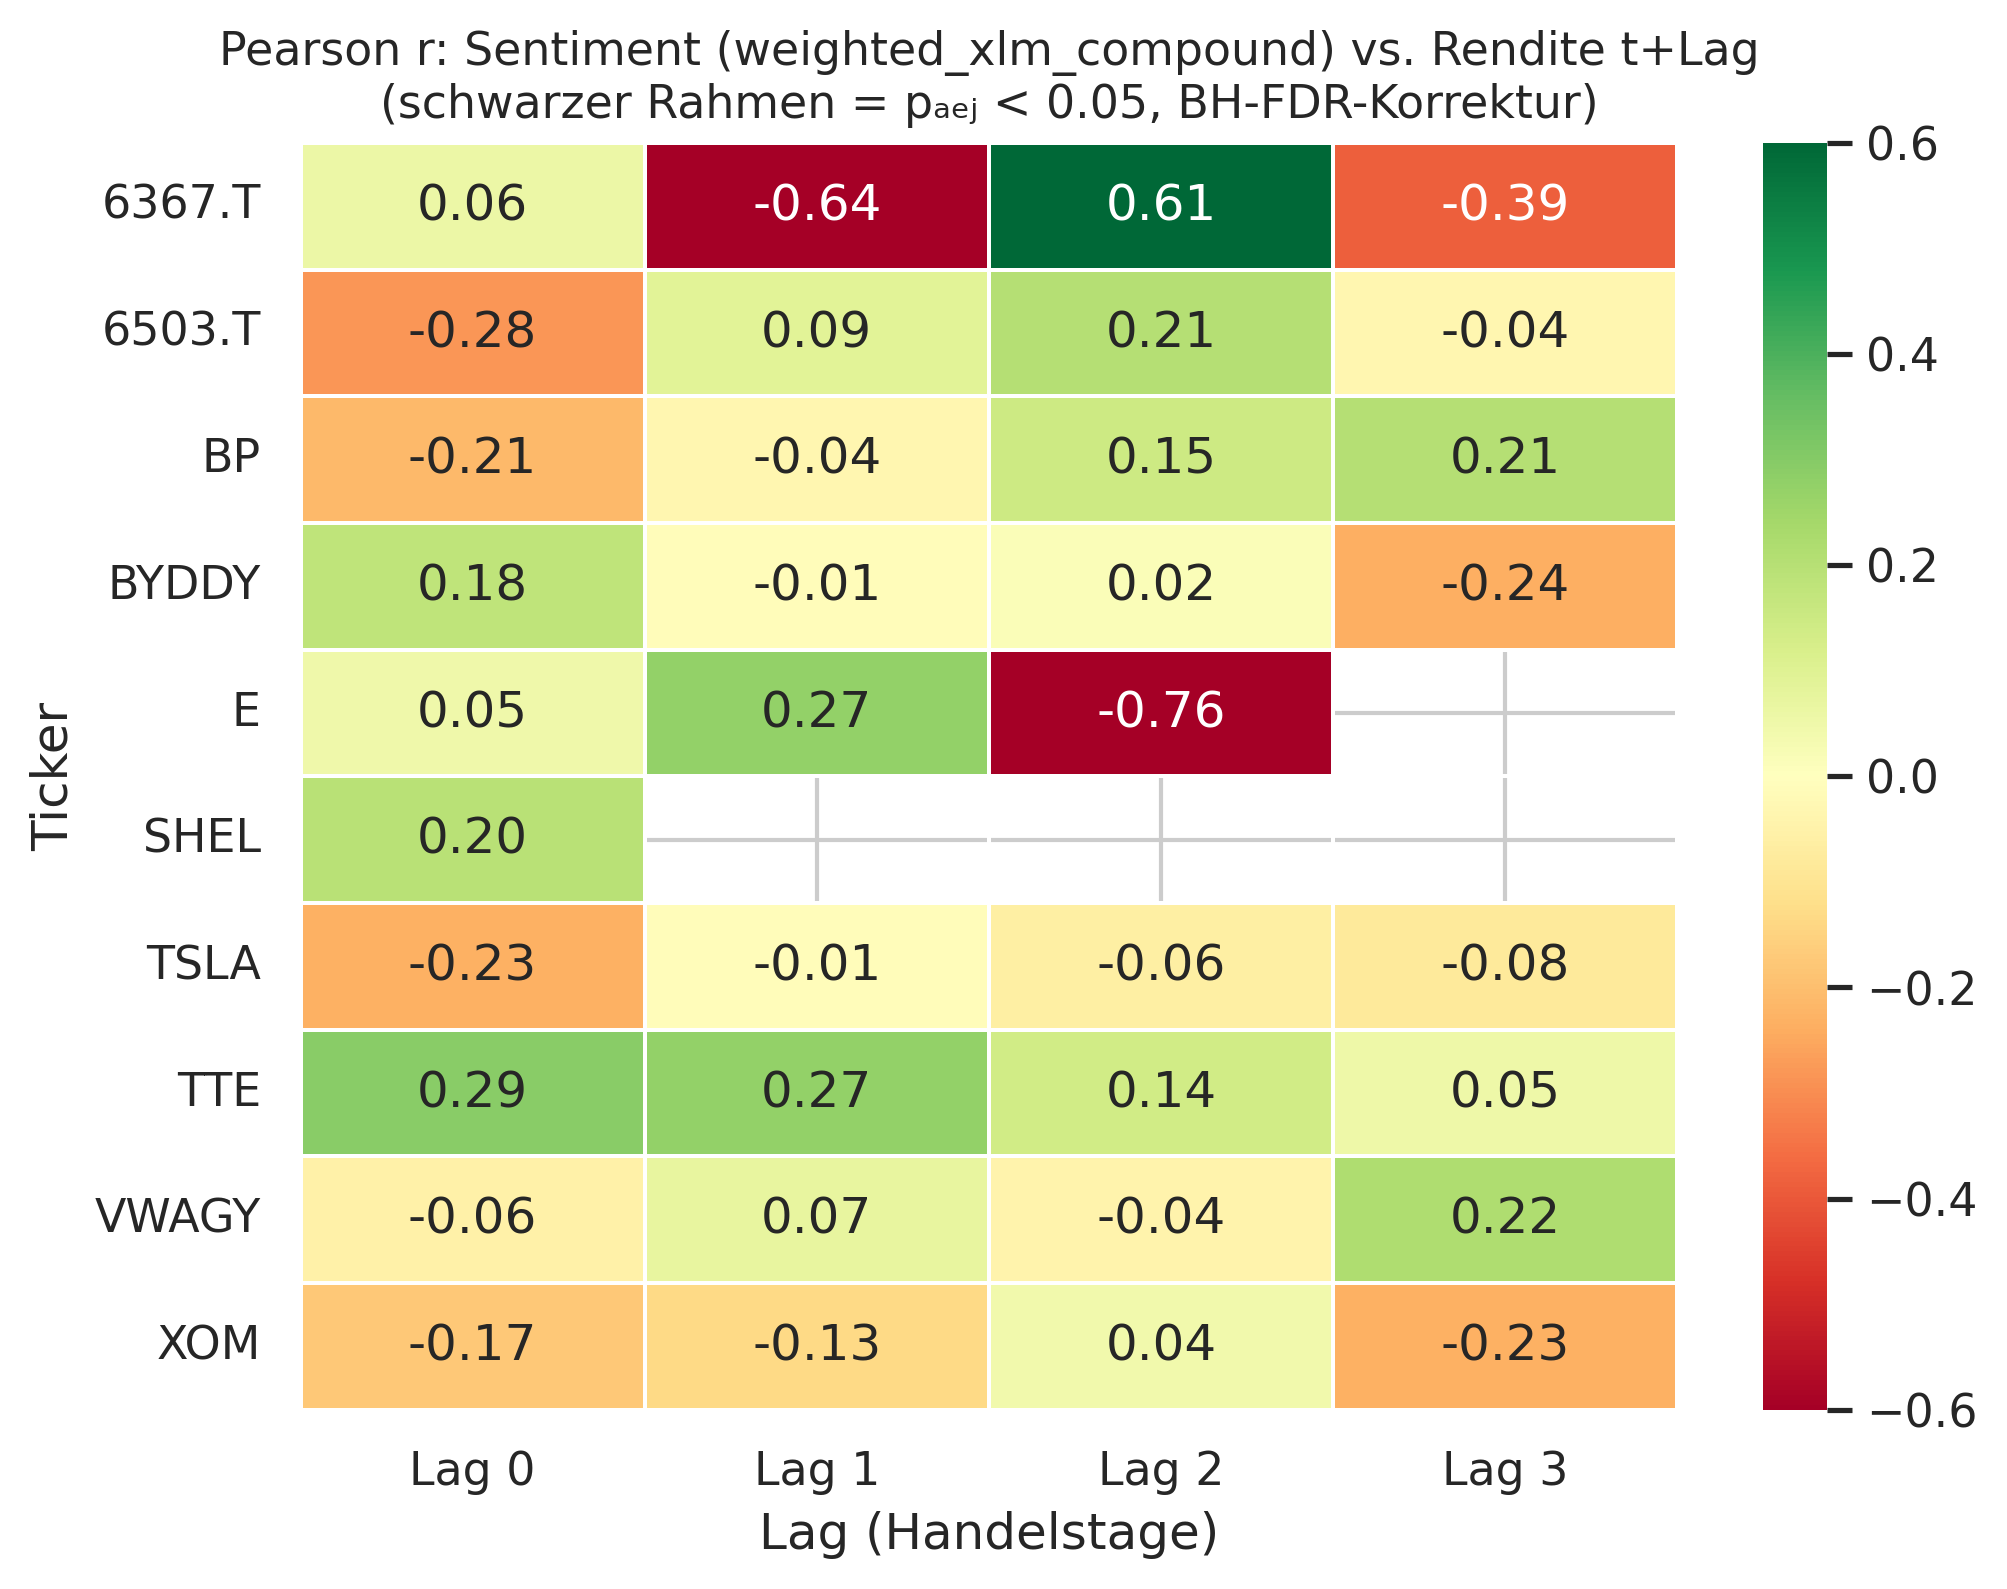
\includegraphics[width=0.72\textwidth]{figures/03_correlation_modeling/01_pearson_heatmap_lags.png}
  \caption{Pearson-Korrelationskoeffizient $r$ zwischen follower-gewichtetem Sentiment am Tag $t$ und Rendite am Tag $t+\text{Lag}$. Da nach BH-FDR-Korrektur kein $p_{\mathrm{adj}} < 0{,}05$ vorliegt, zeigt die Heatmap keine schwarz umrahmten Zellen.}
  \label{fig:pearson_heatmap}
\end{figure}

% ─────────────────────────────────────────────────────────────────────────────
\subsection{Rolling-Korrelation}
\label{subsec:ergebnisse_rolling}

\begin{figure}[H]
  \centering
  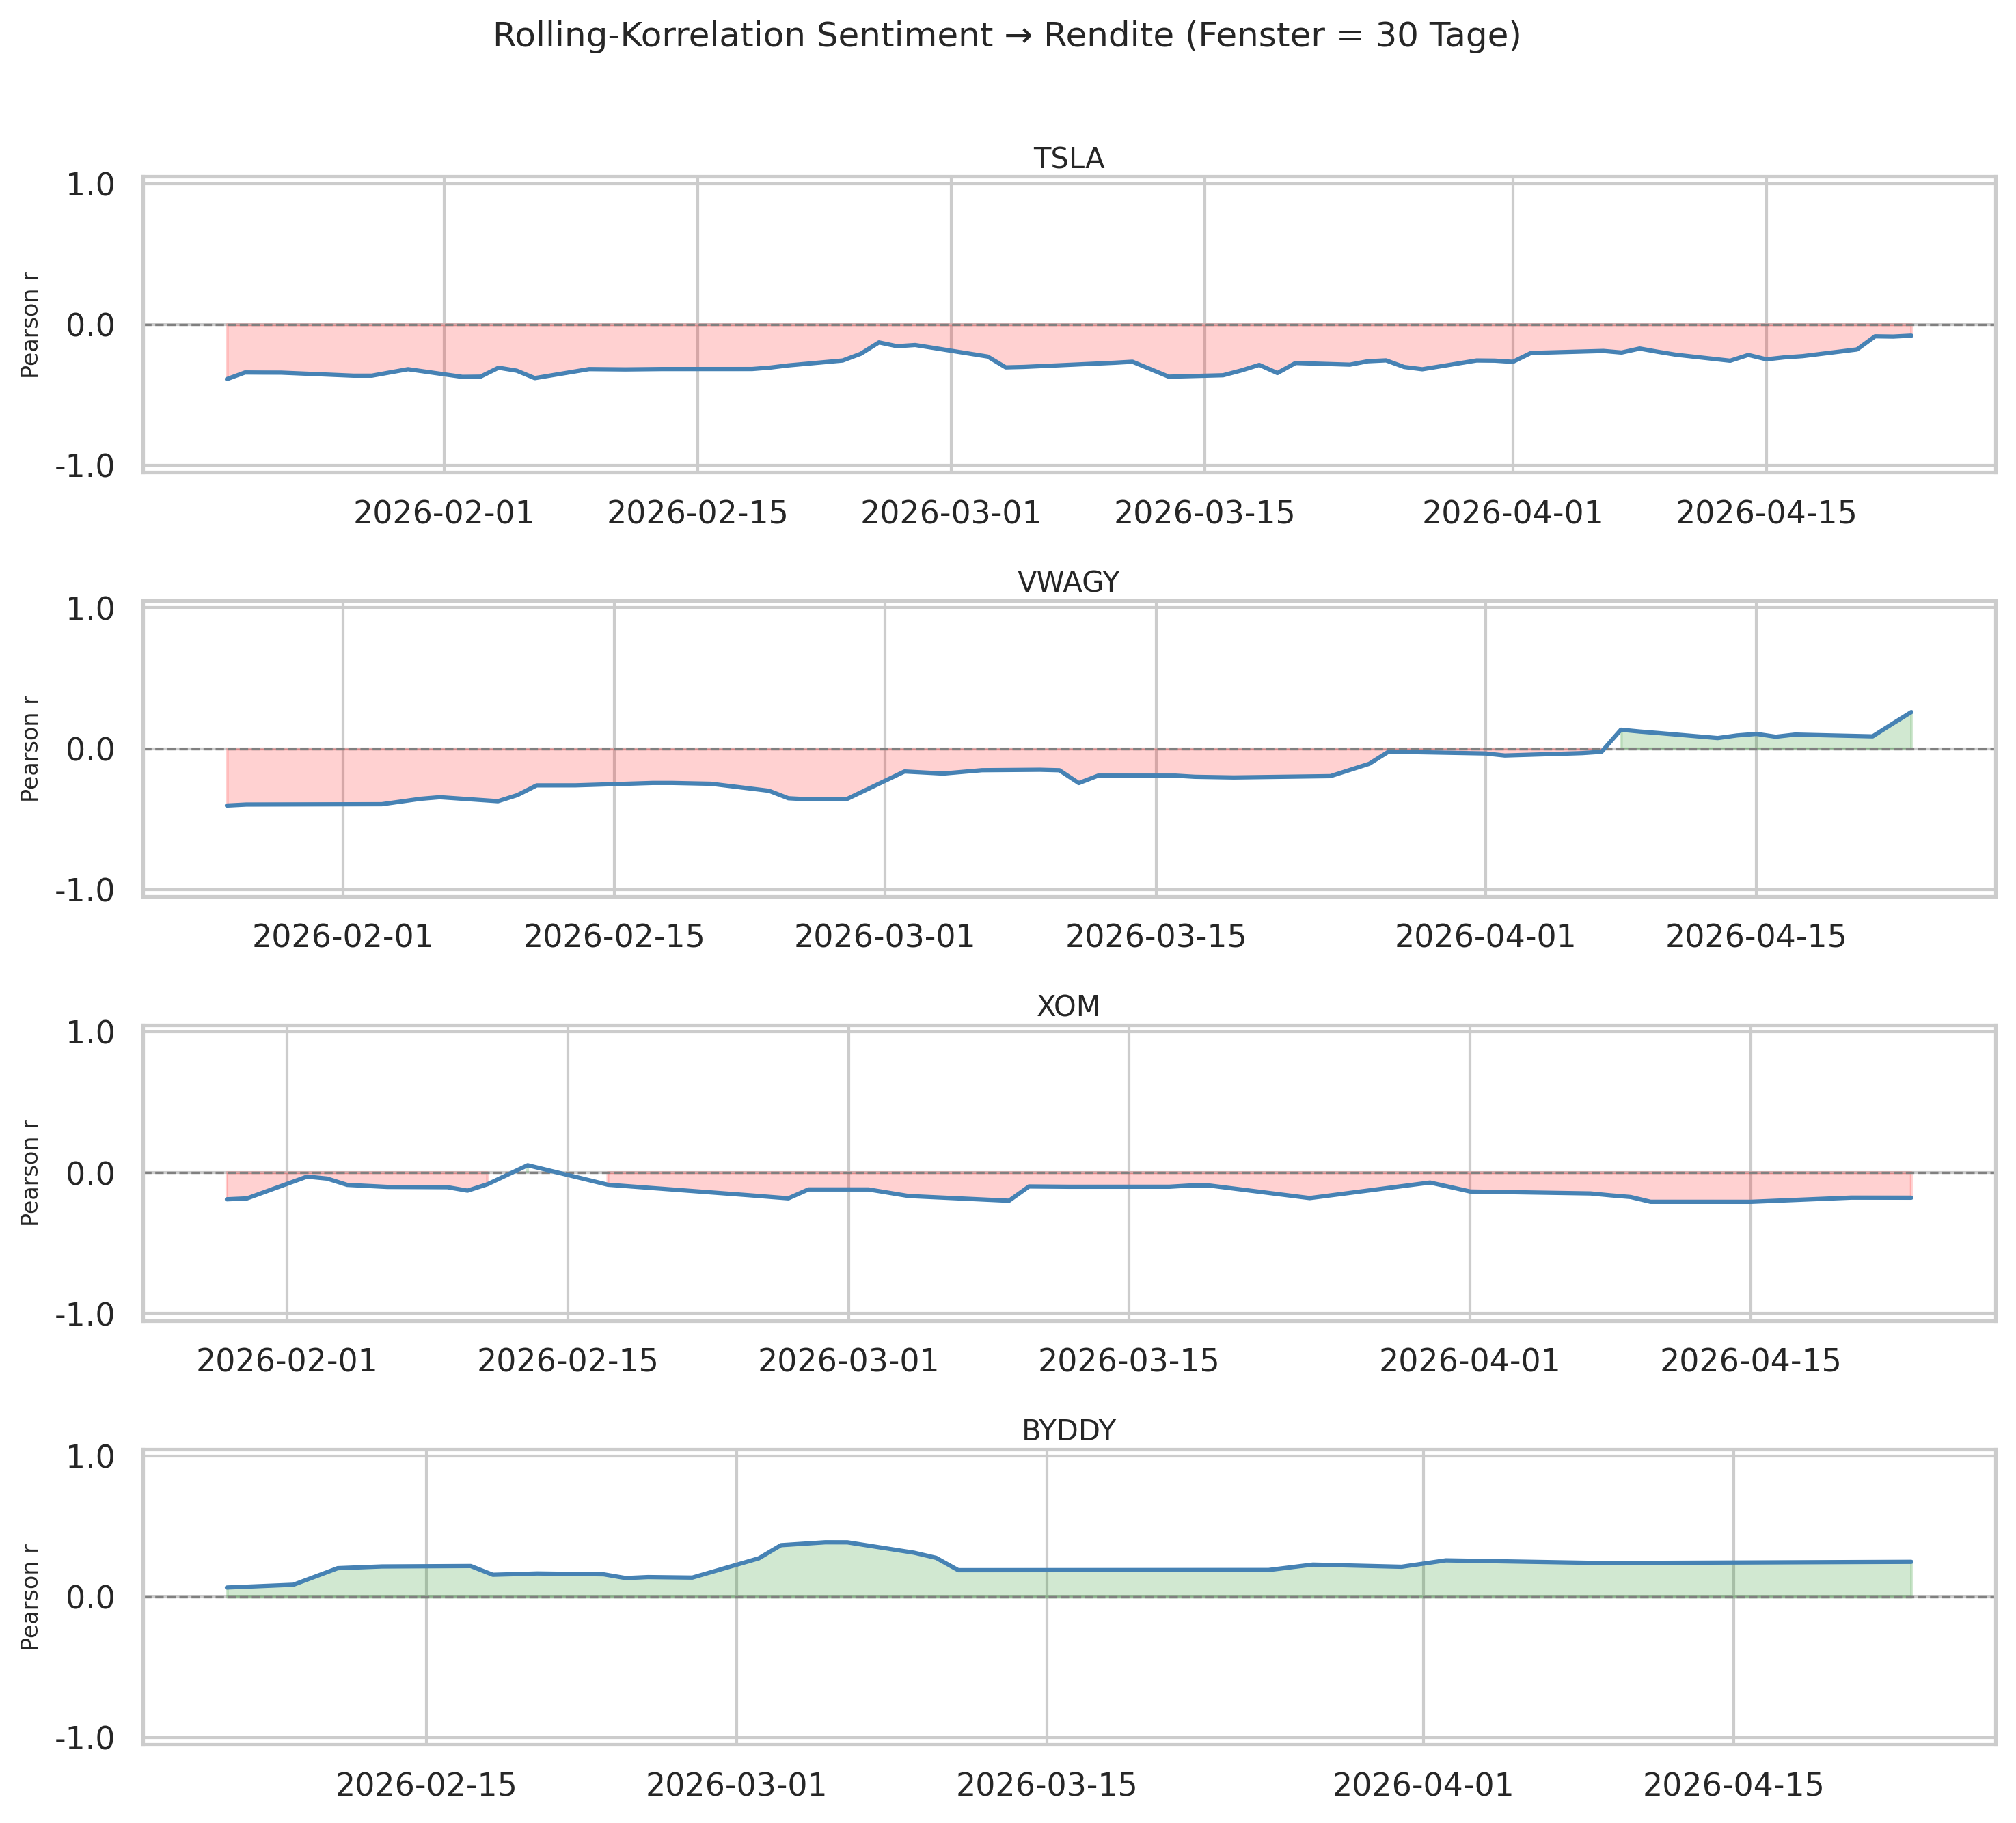
\includegraphics[width=0.9\textwidth]{figures/03_correlation_modeling/02_rolling_correlation.png}
  \caption{Rolling-Korrelation Sentiment $\rightarrow$ Rendite (gleitendes Fenster: 30 Handelstage, Minimum: 10 Punkte) für TSLA, VWAGY, XOM und BYDDY. Grüne Flächen zeigen positive, rote Flächen negative Korrelationsphasen.}
  \label{fig:rolling}
\end{figure}

Die Rolling-Korrelation konnte für vier Ticker berechnet werden: TSLA, VWAGY, XOM und BYDDY. Für alle vier Ticker wechselte das Vorzeichen der Korrelation mehrfach über den Beobachtungszeitraum. Stabile Phasen mit durchgehend positivem oder negativem Zusammenhang waren nicht erkennbar. Dies deutet darauf hin, dass selbst punktuell beobachtbare Zusammenhänge zeitlich nicht robust sind.

% ─────────────────────────────────────────────────────────────────────────────
\subsection{Granger-Kausalitätstest}
\label{subsec:ergebnisse_granger}

Für die vier Ticker mit mindestens 30 Beobachtungen (TSLA, VWAGY, XOM, BYDDY) wurden Granger-Kausalitätstests in beiden Richtungen für Lags 1 bis 3 durchgeführt. Keiner der berechneten F-Test-$p$-Werte unterschritt die Signifikanzschwelle von 0.05. Tabelle~\ref{tab:granger} zeigt die $p$-Werte für die Richtung Sentiment $\rightarrow$ Rendite.

\begin{table}[H]
\centering
\caption{Granger-Kausalitätstest: $p$-Werte (Sentiment $\rightarrow$ Rendite, F-Test)}
\label{tab:granger}
\begin{tabular}{lrrr}
\toprule
\textbf{Ticker} & \textbf{Lag 1} & \textbf{Lag 2} & \textbf{Lag 3} \\
\midrule
TSLA  & 0.957 & 0.658 & 0.602 \\
VWAGY & 0.656 & 0.842 & 0.444 \\
XOM   & 0.544 & 0.712 & 0.349 \\
BYDDY & 0.901 & 0.918 & 0.757 \\
\bottomrule
\end{tabular}
\end{table}

Die $p$-Werte lagen durchgängig deutlich über 0.30, teilweise über 0.90. Es konnte kein Hinweis gefunden werden, dass vergangenes Sentiment die Rendite besser vorhersagt als die Rendite allein.

\begin{figure}[H]
  \centering
  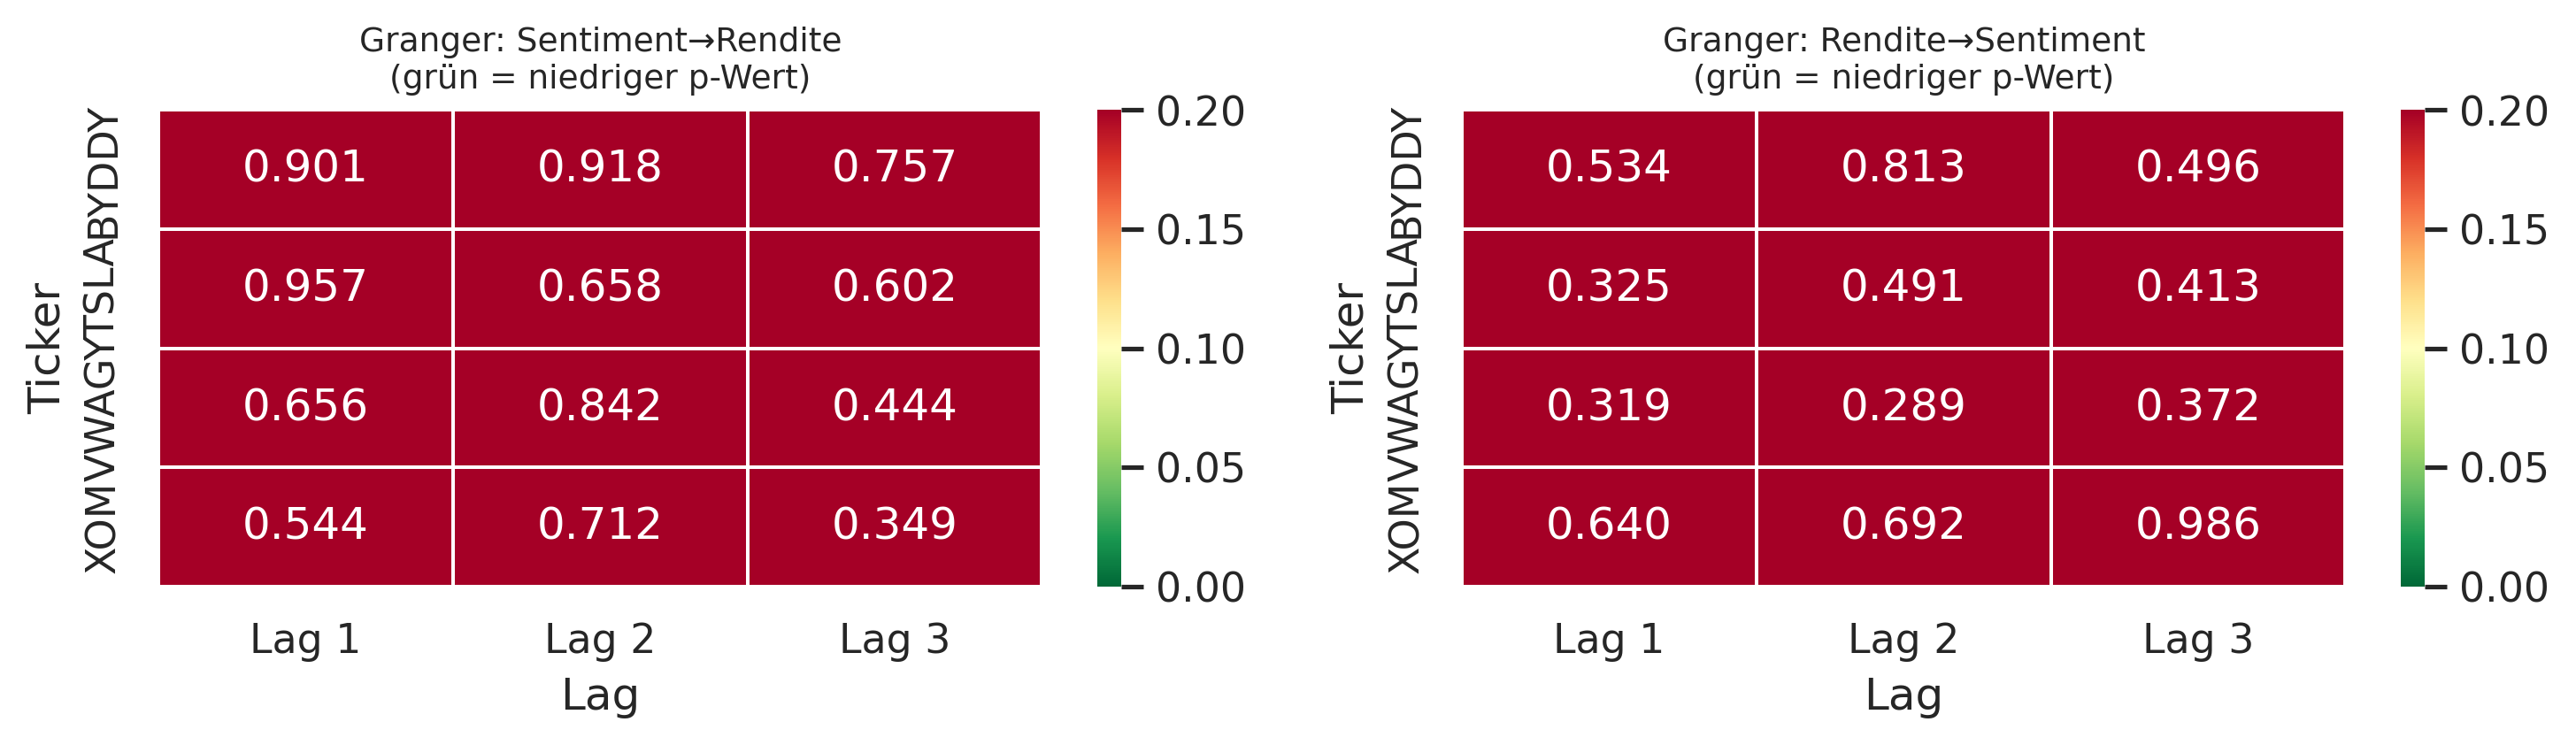
\includegraphics[width=0.85\textwidth]{figures/03_correlation_modeling/03_granger_heatmaps.png}
  \caption{Granger-Kausalitätstest $p$-Werte (F-Test) für beide Richtungen: Sentiment $\rightarrow$ Rendite (links) und Rendite $\rightarrow$ Sentiment (rechts). Grüne Farbe entspricht niedrigen $p$-Werten; kein Wert unterschreitet $p = 0.05$.}
  \label{fig:granger_heatmap}
\end{figure}

% ─────────────────────────────────────────────────────────────────────────────
\subsection{Event-Study}
\label{subsec:ergebnisse_event}

Die Event-Study identifizierte für sechs Ticker ausreichend Ereignisse (mindestens 5 je Richtung). Tabelle~\ref{tab:events} zeigt die Anzahl der positiven und negativen Ereignisse je Ticker.

\begin{table}[H]
\centering
\caption{Event-Study: Anzahl der Ereignisse je Ticker und Richtung}
\label{tab:events}
\begin{tabular}{lrr}
\toprule
\textbf{Ticker} & \textbf{Positive Ereignisse} & \textbf{Negative Ereignisse} \\
\midrule
TSLA  & 11 &  9 \\
VWAGY &  5 &  9 \\
XOM   &  8 &  8 \\
BYDDY &  6 &  5 \\
BP    &  0 &  5 \\
TTE   &  5 &  0 \\
\bottomrule
\end{tabular}
\end{table}

\begin{figure}[H]
  \centering
  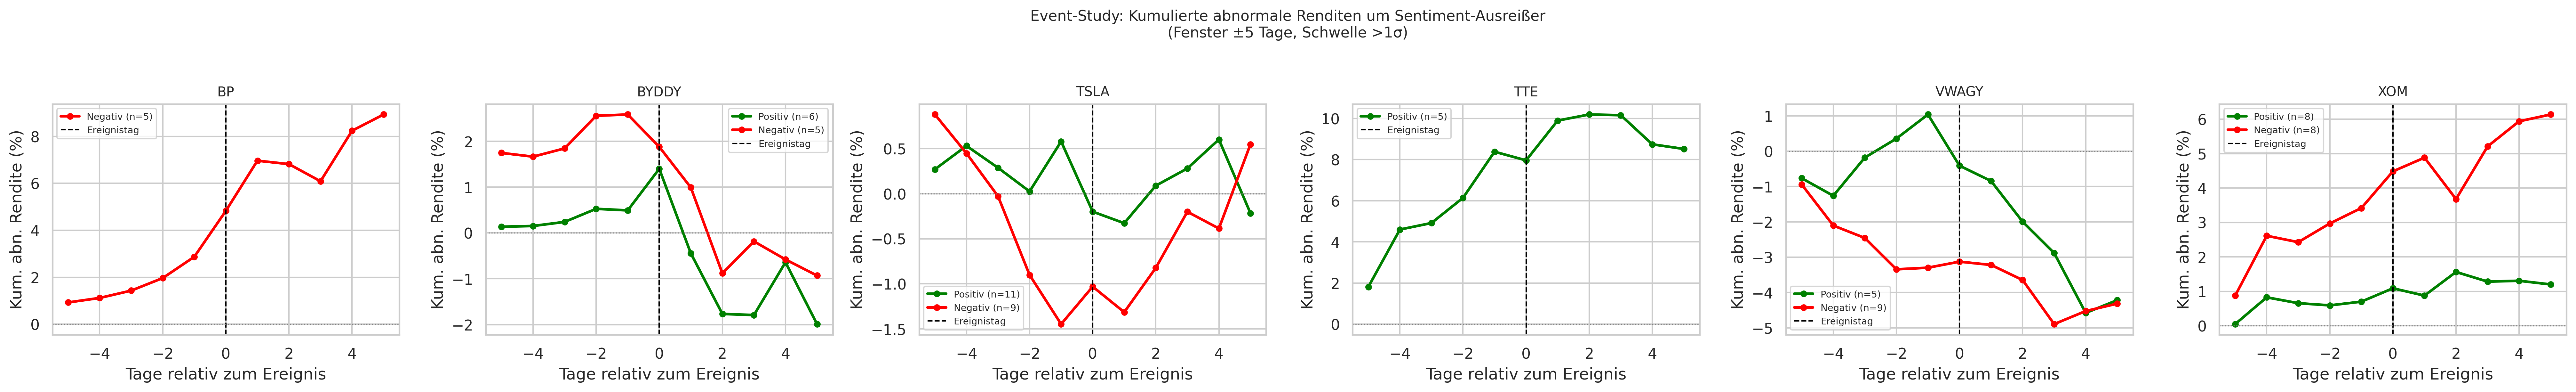
\includegraphics[width=\textwidth]{figures/03_correlation_modeling/04_event_study_car.png}
  \caption{Kumulierte abnormale Renditen (CAR) um Sentiment-Ausrei\ss ertage ($>\!1\sigma$), Fenster $\pm$5 Handelstage, Benchmark: S\&P\,500-Index (\textasciicircum GSPC). Grüne Linien = positive Ereignisse, rote Linien = negative Ereignisse.}
  \label{fig:event_study}
\end{figure}

Die CAR-Profile zeigten keine einheitliche Richtung. Für einzelne Ticker (z.\,B.\ TSLA) war ein gewisses Muster rund um den Ereignistag erkennbar, jedoch ohne statistisch signifikante oder unternehmenübergreifend konsistente Struktur. Positive Sentiment-Ereignisse führten nicht regelmäßig zu positiven abnormalen Renditen -- und umgekehrt.
